\documentclass[12pt]{article}

\usepackage[dvipsnames]{xcolor}
\usepackage{../../packages/shared}
\usepackage{../../packages/misc_commands}
% =========================
% Causal Structure Diagrams
% =========================
\definecolor{obs_outline}{RGB}{51,157,215}
\definecolor{obs_fill}{RGB}{222,253,255}
\definecolor{obs_text}{RGB}{0,0,0}
\definecolor{lat_outline}{RGB}{251,141,54}
\definecolor{cause}{RGB}{30, 0, 30}
\definecolor{lat_fill}{RGB}{255,213,153}
\definecolor{lat_text}{RGB}{0,0,0}
\tikzset{square/.style={regular polygon,regular polygon sides=4}}
\tikzset{triangle/.style={regular polygon,regular polygon sides=3}}
\tikzset{observed/.style={obs_text, align=center, triangle, thick, draw=obs_outline, fill=obs_fill, inner sep=-0.2em, text width=1.5em}}
\tikzset{latent/.style={lat_text, align=center, circle, thick, draw=lat_outline, fill=lat_fill, text width=1.5em, inner sep=0.2em}}
\tikzset{fade/.style={opacity=0.2}}
\tikzset{unfade/.style={opacity=1.0}}
% TikZ stile to apply keys only on specific beamer overlays
% onslide=<overlay spec>{key=value, key=value, ...}
\tikzset{onslide/.code args={<#1>#2}{%
  \only<#1>{\pgfkeysalso{#2}}%
}}
\providecommand{\p}[1]{#1}
% \tikzset{cause/.style={mid arrow/.style={postaction={decorate,decoration={markings, mark=at position .5 with {\arrow[#1]{stealth}}}}},}}
\tikzset{
    % style to apply some styles to each segment of a path
    on each segment/.style={
        decorate,
        decoration={
            show path construction,
            moveto code={},
            lineto code={
                \path [#1]
                (\tikzinputsegmentfirst) -- (\tikzinputsegmentlast);
            },
            curveto code={
                \path [#1] (\tikzinputsegmentfirst)
                .. controls
                (\tikzinputsegmentsupporta) and (\tikzinputsegmentsupportb)
                ..
                (\tikzinputsegmentlast);
            },
            closepath code={
                \path [#1]
                (\tikzinputsegmentfirst) -- (\tikzinputsegmentlast);
            },
        },
    },
    % style to add an arrow in the middle of a path
    mid arrow/.style={postaction={decorate,decoration={
                markings,
                mark=at position .6 with {\arrow[scale=1.5, cause]{stealth}}
            }}},
}
% =========================
% ========================= % Causal structure formatting for tikz

\begin{document}

    \textbf{Rosset Variation:}\\

    Considering the \term{WagonWheel} inflation depicted below,

    \begin{center}
        \scalebox{1.0}{\newcommand{\ift}{2.3}
\newcommand{\hvspoke}{0.8}
\newcommand{\diagspoke}{1.1}
\begin{tikzpicture}[scale=2]
    \begin{scope}[every node/.style=observed]
        \node (A1) at ({0}, {\hvspoke}) {$\p{A}_1$};
        \node (A2) at ({0}, {-\hvspoke}) {$\p{A}_2$};
        \node (B1) at ({-\hvspoke}, {0}) {$\p{B}_1$};
        \node (B2) at ({\hvspoke}, {0}) {$\p{B}_2$};
        \node (C1) at ({+\diagspoke}, {+\diagspoke}) {$\p{C}_1$};
        \node (C2) at ({+\diagspoke}, {-\diagspoke}) {$\p{C}_2$};
        \node (C3) at ({-\diagspoke}, {-\diagspoke}) {$\p{C}_3$};
        \node (C4) at ({-\diagspoke}, {+\diagspoke}) {$\p{C}_4$};
    \end{scope}
    \begin{scope}[every node/.style=latent]
        \node (Y1) at (0, 0) {$\p{Y}_1$};
        \node (X1) at ({0}, {2*\hvspoke}) {$\p{X}_1$};
        \node (Z1) at ({2*\hvspoke}, {0}) {$\p{Z}_1$};
        \node (X2) at ({0}, {-2*\hvspoke}) {$\p{X}_2$};
        \node (Z2) at ({-2*\hvspoke}, {0}) {$\p{Z}_2$};
    \end{scope}
    \begin{scope}[every path/.style={draw=cause, thick}]
        \path[postaction={on each segment={mid arrow}}]
        % Y1
        (Y1) -- (A1)
        (Y1) -- (A2)
        (Y1) -- (B1)
        (Y1) -- (B2)
        % X1
        (X1) -- (C1)
        (X1) -- (C4)
        (X1) -- (A1)
        % Z1
        (Z1) -- (C1)
        (Z1) -- (C2)
        (Z1) -- (B2)
        % X2
        (X2) -- (C2)
        (X2) -- (C3)
        (X2) -- (A2)
        % Z2
        (Z2) -- (C4)
        (Z2) -- (C3)
        (Z2) -- (B1)
        ;
    \end{scope}
\end{tikzpicture}}
    \end{center}

    And the usual \term{Fritz distribution},

    \begin{center}
        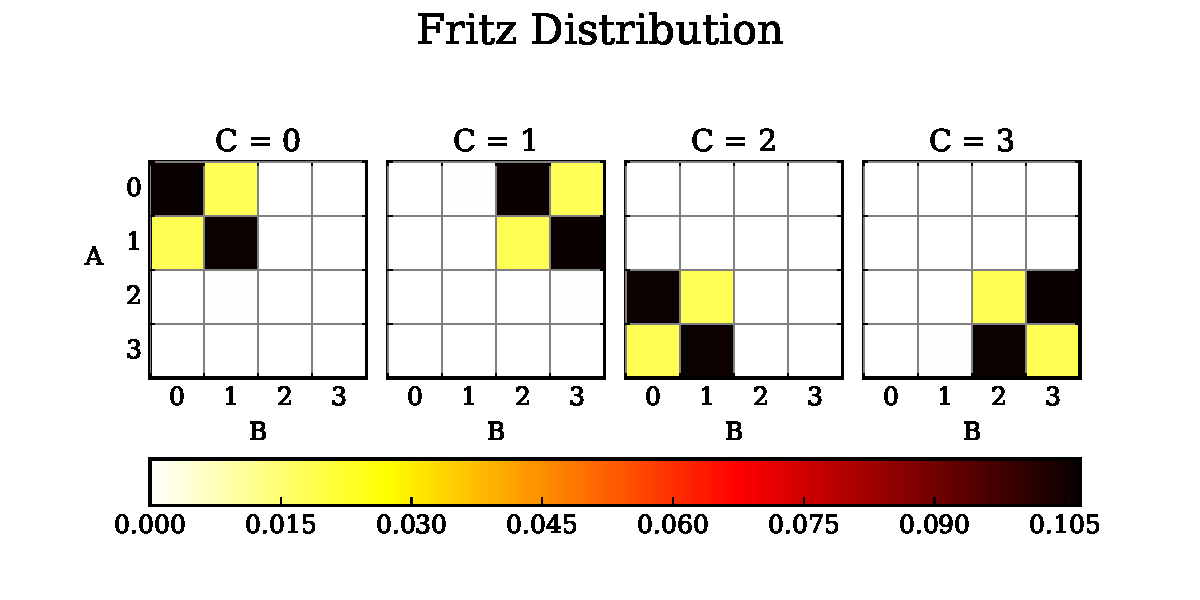
\includegraphics[width=\linewidth]{../../figures/distributions/fritz_dist_plotted.pdf}
    \end{center}

    The maximal pre-injectable sets are,

    \begin{align*}
        \bc{\bc{A_2, B_1, C_3}, \bc{C_1}} \\
        \bc{\bc{A_1, B_1, C_4}, \bc{C_2}} \\
        \bc{\bc{A_1, B_2, C_1}, \bc{C_3}} \\
        \bc{\bc{A_2, B_2, C_2}, \bc{C_4}} \\
    \end{align*}

    And they define an incidence matrix that is $1024 \times 65,536$. Using the \term{Definite Extension Procedure} to first order (i.e. single antecedent) I can derive the following representative inequality:

    \begin{gather*}
    P_{ABC}(000)P_{C}(3) \\
    \leq \\
    2P_{ABC}(203)P_{C}(0) + 2P_{ABC}(303)P_{C}(0) + P_{ABC}(003)P_{C}(0) + P_{ABC}(013)P_{C}(0) + \\
    P_{ABC}(020)P_{C}(2) + P_{ABC}(022)P_{C}(2) + P_{ABC}(023)P_{C}(0) + P_{ABC}(023)P_{C}(2) + \\
    P_{ABC}(030)P_{C}(2) + P_{ABC}(031)P_{C}(2) + P_{ABC}(032)P_{C}(2) + P_{ABC}(033)P_{C}(0) + \\
    P_{ABC}(033)P_{C}(2) + P_{ABC}(103)P_{C}(0) + P_{ABC}(113)P_{C}(0) + P_{ABC}(123)P_{C}(0) + \\
    P_{ABC}(133)P_{C}(0) + P_{ABC}(200)P_{C}(0) + P_{ABC}(200)P_{C}(1) + P_{ABC}(200)P_{C}(2) + \\
    P_{ABC}(200)P_{C}(3) + P_{ABC}(201)P_{C}(0) + P_{ABC}(201)P_{C}(1) + P_{ABC}(201)P_{C}(2) + \\
    P_{ABC}(201)P_{C}(3) + P_{ABC}(203)P_{C}(1) + P_{ABC}(203)P_{C}(2) + P_{ABC}(203)P_{C}(3) + \\
    P_{ABC}(213)P_{C}(0) + P_{ABC}(223)P_{C}(0) + P_{ABC}(300)P_{C}(0) + P_{ABC}(300)P_{C}(1) + \\
    P_{ABC}(300)P_{C}(2) + P_{ABC}(300)P_{C}(3) + P_{ABC}(301)P_{C}(0) + P_{ABC}(301)P_{C}(1) + \\
    P_{ABC}(301)P_{C}(2) + P_{ABC}(301)P_{C}(3) + P_{ABC}(302)P_{C}(1) + P_{ABC}(303)P_{C}(1) + \\
    P_{ABC}(303)P_{C}(2) + P_{ABC}(303)P_{C}(3) + P_{ABC}(313)P_{C}(0) \\
    \end{gather*}

    That witnesses the Fritz distribution with violation,
    \[ -0.0129428304698 \]
    \textit{Quite interestingly}, all my numerical attempts to violate further are fruitless (only improving on the violation in the $6$-th decimal place $-0.0129437678359$). Therefore, it seems that the Fritz distribution is a local minima of this inequality! This inequality also suffers from the global minima issues; any significant deviation from parameters that generate the Fritz distribution results in a null result (the optimization tends toward inequality saturation).\\

    Regarding noise, it seems that this inequality is \textit{less robust} to noise than some of the ones generated via the web inflation (crossing the saturation point around $\ep \approx 0.07$ instead of $\ep \approx 0.08$),

    \begin{center}
        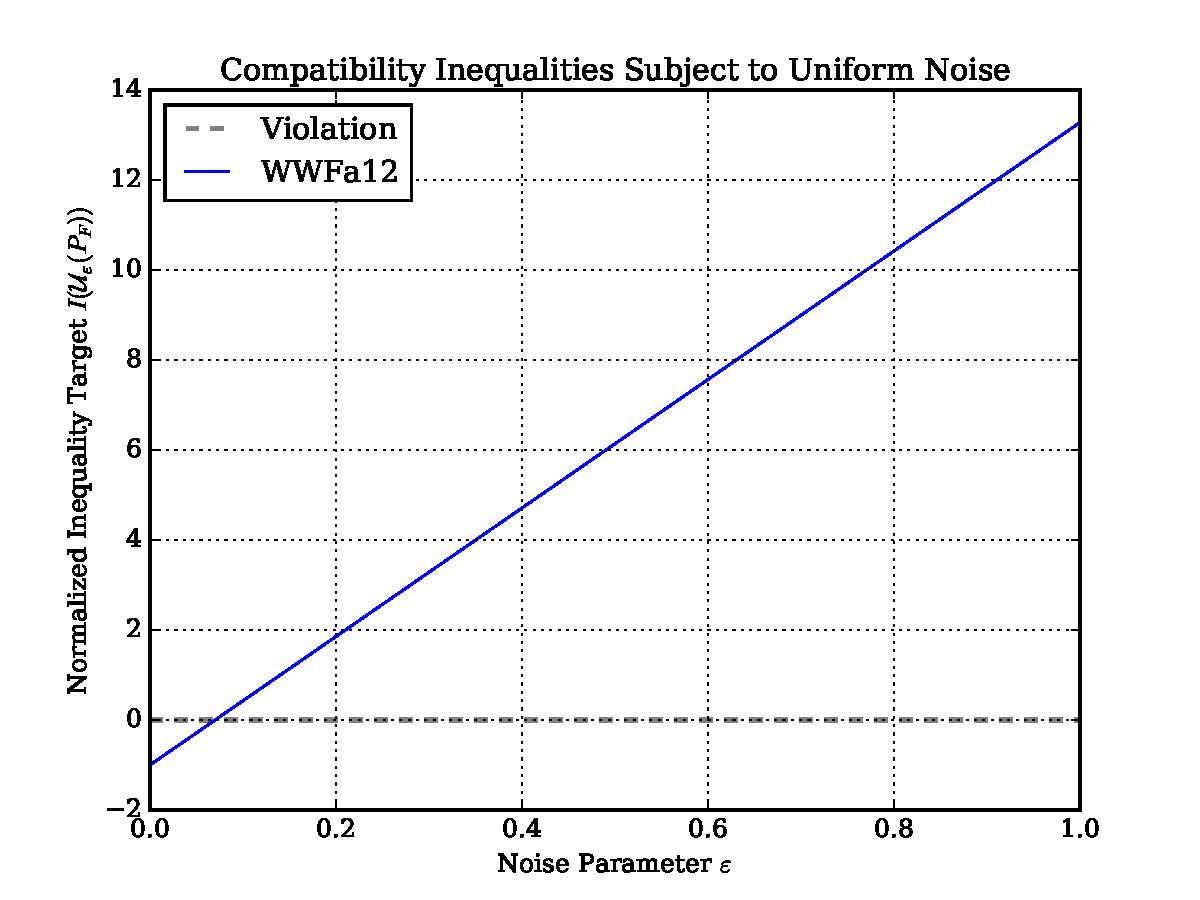
\includegraphics[width=\linewidth]{../../figures/noise/wagon_wheel_12.pdf}
    \end{center}

    More importantly, you asked about the \term{Rosset Variation} to the Fritz distribution where $C$ announces $A\tsb{in} \cdot B\tsb{in}$ instead of the usual $\bc{A\tsb{in},B\tsb{in}}$

    \begin{center}
        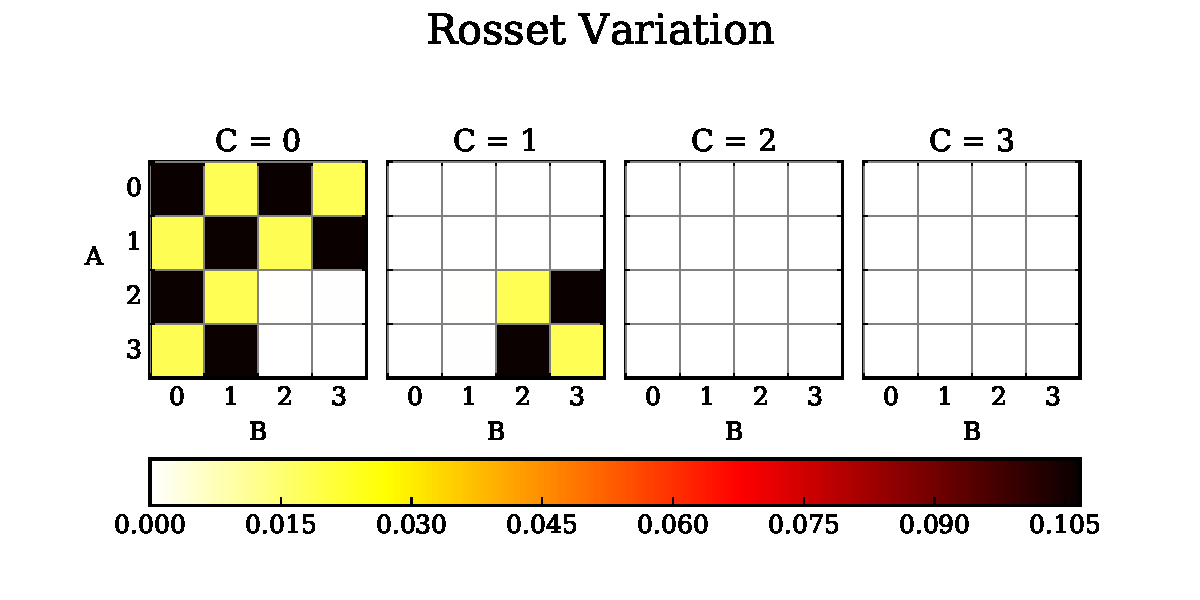
\includegraphics[width=\linewidth]{../../figures/distributions/rosset_variation_plotted.pdf}
    \end{center}

    \textit{Very interestingly}, it turns out that this distribution \textbf{can not} be witnessed by first order inequalities! This is so surprising to me that I in doubt; Did you manage to witness this as a first order inequality? If so, then there is something broken in my code.\\

    If I am correct, this suggests something very interesting. Additionally, I am interested in checking this Rosset Variation against the large/web inflation in order to see if first order inequalities can be found there. I have been reluctant to do this myself as my laptop does not possess the computing requirements and my desktop machine at home can be unreliable. Let me know if this is worth pursuing. Additionally, I will be implementing the definition extension procedure in full over the next few weeks so it will be interesting to see at what order the Rosset Variation can be witnessed. \\

    \textbf{Compactifying Inequalities:}\\

    In addition, I attempted to find a way to compactify the notation/terms present in some of the inequalities we have found thus far. I attempted to write some code to this but made insignificant progress. The process is still very manual and the compactified inequalities are still hard to interpret. For example, the inequality presented above can be written as:

    \begin{gather*}
        P_{ABC}(000)P_{C}(3) + P_{ABC}(021)P_{C}(2) + \\
        P_{ABC}(202) + P_{ABC}(302) + \\
        P_{ABC}(233)P_{C}(0) + P_{AC}(33)P_{C}(0) \\
        \leq \\ P_{ABC}(303)P_{C}(0) + P_{ABC}(313)P_{C}(0) + P_{ABC}(302)P_{C}(1) + \\
        P_{AB}(02)P_{C}(2) + P_{AB}(03)P_{C}(2) + P_{AB}(20) + P_{AB}(30) + \\
        P_{C}(3)P_{C}(0)
    \end{gather*}

    Of course, this inequality is the result of a \textit{canonical minimalization}. Without minimalizing the inequalities (i.e. keeping all of the zero-weighted terms pursuant to the Fritz distribution) one obtains,

    \begin{gather*}
        P_{ABC}(000)P_{C}(3) + P_{ABC}(003)P_{C}(0) + P_{ABC}(103)P_{C}(0) + \\
        P_{ABC}(000) + P_{ABC}(202) + P_{ABC}(302) + P_{ABC}(100) \\
        \leq \\
        P_{B}(0) + \\
        P_{AC}(03)P_{C}(0) + P_{AC}(13)P_{C}(0) + \\
        P_{AC}(02) + P_{AC}(03) + \\
        P_{BC}(03)P_{C}(0) + \\
        P_{ABC}(011) + P_{ABC}(020) + P_{ABC}(030) + P_{ABC}(001) + \\
        P_{ABC}(031)P_{C}(2) + P_{ABC}(223)P_{C}(0) + P_{ABC}(302)P_{C}(1) + \\
        P_{ABC}(213)P_{C}(0) + P_{ABC}(313)P_{C}(0)
    \end{gather*}

\end{document}